 \documentclass[12pt]{article}
 \usepackage[italian]{babel}

% \usepackage{fontspec}
% \setmainfont{Calibri}

 %setting margins
 \usepackage[margin=2cm,nohead]{geometry}
 \usepackage{circuitikz}
 \usepackage{graphicx}
 \usepackage{tikz}
 \usepackage{booktabs}
 \usepackage{amsmath}
 \usepackage{hyperref}



 \ctikzset{bipoles/thickness=1.2}

 \title{Analisi di un circuito RLC serie in regime sinusoidale}
 \author{Autori: Niccolò Zanotti mat. 970919, Michael Mancini mat. 987056}
 \date{Data di svolgimento: 01/06/2022}

 \begin{document}

 \maketitle
% \hrulefill   %horizontal line

 \section{Abstract}
    In questa esperienza di laboratorio si è analizzato il comportamento di un circuito RLC serie, sottoposto ad una tensione
in regime sinusoidale con pulsazione variabile.
In particolar modo, si è cercato di stimare il valore della frequenza di risonanza, andando a confrontare il comportamento
del circuito per valori della frequenza prossimi
al valore cercato per poi, acquisendo e analizzando i dati relativi alla tensione in entrata e nei rami, verificare
l’andamento atteso dell’ampiezza della tensione.

Le stime più significative della frequenza di risonanza sono $f_0 = (18.95 \pm 0.05) kHz$, valore ottenuto dai parametri
del fit sulla curva dell’ampiezza della resistenza e $f_0 = (19.10 \pm 0.10)kHz$, valore per cui la tensione su di essa
ha fase nulla, compatibili con il valore atteso pari a $f_0 = (19.13 \pm 0.14) kHz$.



 \section{Introduzione}
   In un circuito $RLC$ in regime sinusoidale si assiste al fenomeno fisico della risonanza; in particolare, dati i valori
caratteristici di resistenza,induttanza e capacità del circuito, si osserva tale fenomeno in corrispondenza di un preciso
valore di frequenza, detta,appunto, di risonanza. La larghezza della curva di risonanza è legato al valore del cosiddetto
fattore di qualità $Q$ del circuito determinato dai componenti circuitali utilizzate.
È stato utilizzato un generatore di tensione sinusoidale il cui scopo principale è stato quello di indurre oscillazioni
della corrente all'interno circuito e per valutare la sua risposta in frequenza.

La frequenza di risonanza si ha quando la tensione generata ai capi del circuito oscilla con pulsazione
\begin{equation}\label{eq:res-pulsation}
    \omega_0 = \frac{1}{\sqrt{L C}}
\end{equation}
In corrispondenza di questo valore il comportamento previsto è che la differenza di potenziale ai capi della
resistenza sia in fase con quella ai capi del generatore e che, inoltre, sia massimizzata l'ampiezza di tali segnali
di tensione.
Tale circuito si classifica tra i filtri di tipo "passa banda", ovvero tra quei dispositivi passivi che permettono il
passaggio di frequenze all'interno di un dato intervallo, la cosiddetta banda passante, ed attenua le frequenze al
di fuori di esso.
% #TODO valuta se mettere osservazione sulla corrente
%poichè in un intorno della frequenza di risonanza, la
%corrente che scorre è maggiore, per poi diminuire di ampiezza a mano mano che ci si allontana dalla condizione sopra citata.
%

 \section{Apparato sperimentale}
   



Il circuito utilizzato è composto da una resistore, un induttore e da un condensatore collegati in serie
sulla breadbord della scheda di acquisizione dati NI Elvis II®.
I valori scelti per i componenti sono i seguenti: $R_r = (996.7 \pm 1.4) \ \Omega$, $C = (1.46 \pm 0.01)10^{-9} \ F$,
$L = (47.41 \pm 0.05)10^{-2} H$ con resistenza interna $R_{\text{ind}} = (125.82 \pm 0.16) \ \Omega$. La resistenza interna
del generatore ammonta a $R_{gen} = 50 \Omega$.
Avendo utilizzato il multimetro digitale di ELVIS II per effettuare le precedenti misurazioni sono state calcolate le
incertezze in accordo con quanto riportato sulla scheda tecnica di tale strumento. Si è valutata l'entità delle possibili
fluttuazioni statistiche mediante misurazioni ripetute per poi confrontare i dati ottenuti con i precedenti. Sono risultate
essere predominanti le incertezze standard. %#TODO come cazzo le chiamo?


I valori precedenti sono stati scelti in maniera tale da ottenere
un fattore di qualità $Q$ ragionevole per una buona osservazione del fenomeno della risonanza. %#TODO commento su Q
%#TODO osservcazione sample rate elvis sulla scelta dei valori

I capi di ogni componente, cosi come gli estremi del circuito, illustrato in Figura \ref{fig:circuit}, sono stati collegati
ad un canale della scheda per poter eseguire la lettura dei valori di ampiezza e fase della tensione su di essi.
Le suddette misure sono state ottenute tramite l'utilizzo del subVI “Extract Single Tone Information” del software di acquisizione
\emph{LabView}.

Per realizzare questa esperienza di laboratorio sono stati raccolti $500$ campioni a frequenza costante in varie condizioni
con una frequenza di $250000$ campioni al secondo, poi, effettuando uno sweep di frequenza, si sono raccolti dati ad
intervalli di $50Hz$ fra $5kHz$ e $35KHz$. %#TODO non proprio cosi uguale

    \begin{figure}
        \centering
        \begin{circuitikz}
            % Circuit
            \draw[line width=0.7]
            (2,7) to [sinusoidal voltage source, l_=$V_S$] (2,1)
            (2,7) to [resistor, l_=$R$]  ++(8,0)to [inductor, l_=$L$] ++(0,-6) to [capacitor,n=cap] +(-8,0) (cap.s) node[above]{$C$};
            \draw[line width=0.7]
            (3,3) to[short,*-] (2,3);
            \draw[line width=0.7]
            (3,5) to[short,*-] (2,5);
            \draw[line width=0.7]
            (5,6) to[short,*-] (5,7);
            \draw[line width=0.7]
            (7,6) to[short,*-] (7,7);
            \draw[line width=0.7]
            (9,5) to[short,*-] (10,5);
            \draw[line width=0.7]
            (9,3) to[short,*-] (10,3);
            \draw[line width=0.7]
            (5,2) to[short,*-] (5,1);
            \draw[line width=0.7]
            (7,2) to[short,*-] (7,1);
            % Grid
% 		\draw[help lines] (0,0) grid (10,10)	;
        \end{circuitikz}
        \caption{\emph{Schema del circuito realizzato.}}
        \label{fig:circuit}
    \end{figure}


 \section{Analisi dei risultati}
   \subsection{Osservazione qualitativa degli andamenti}

\begin{figure}[h]
    \centering
    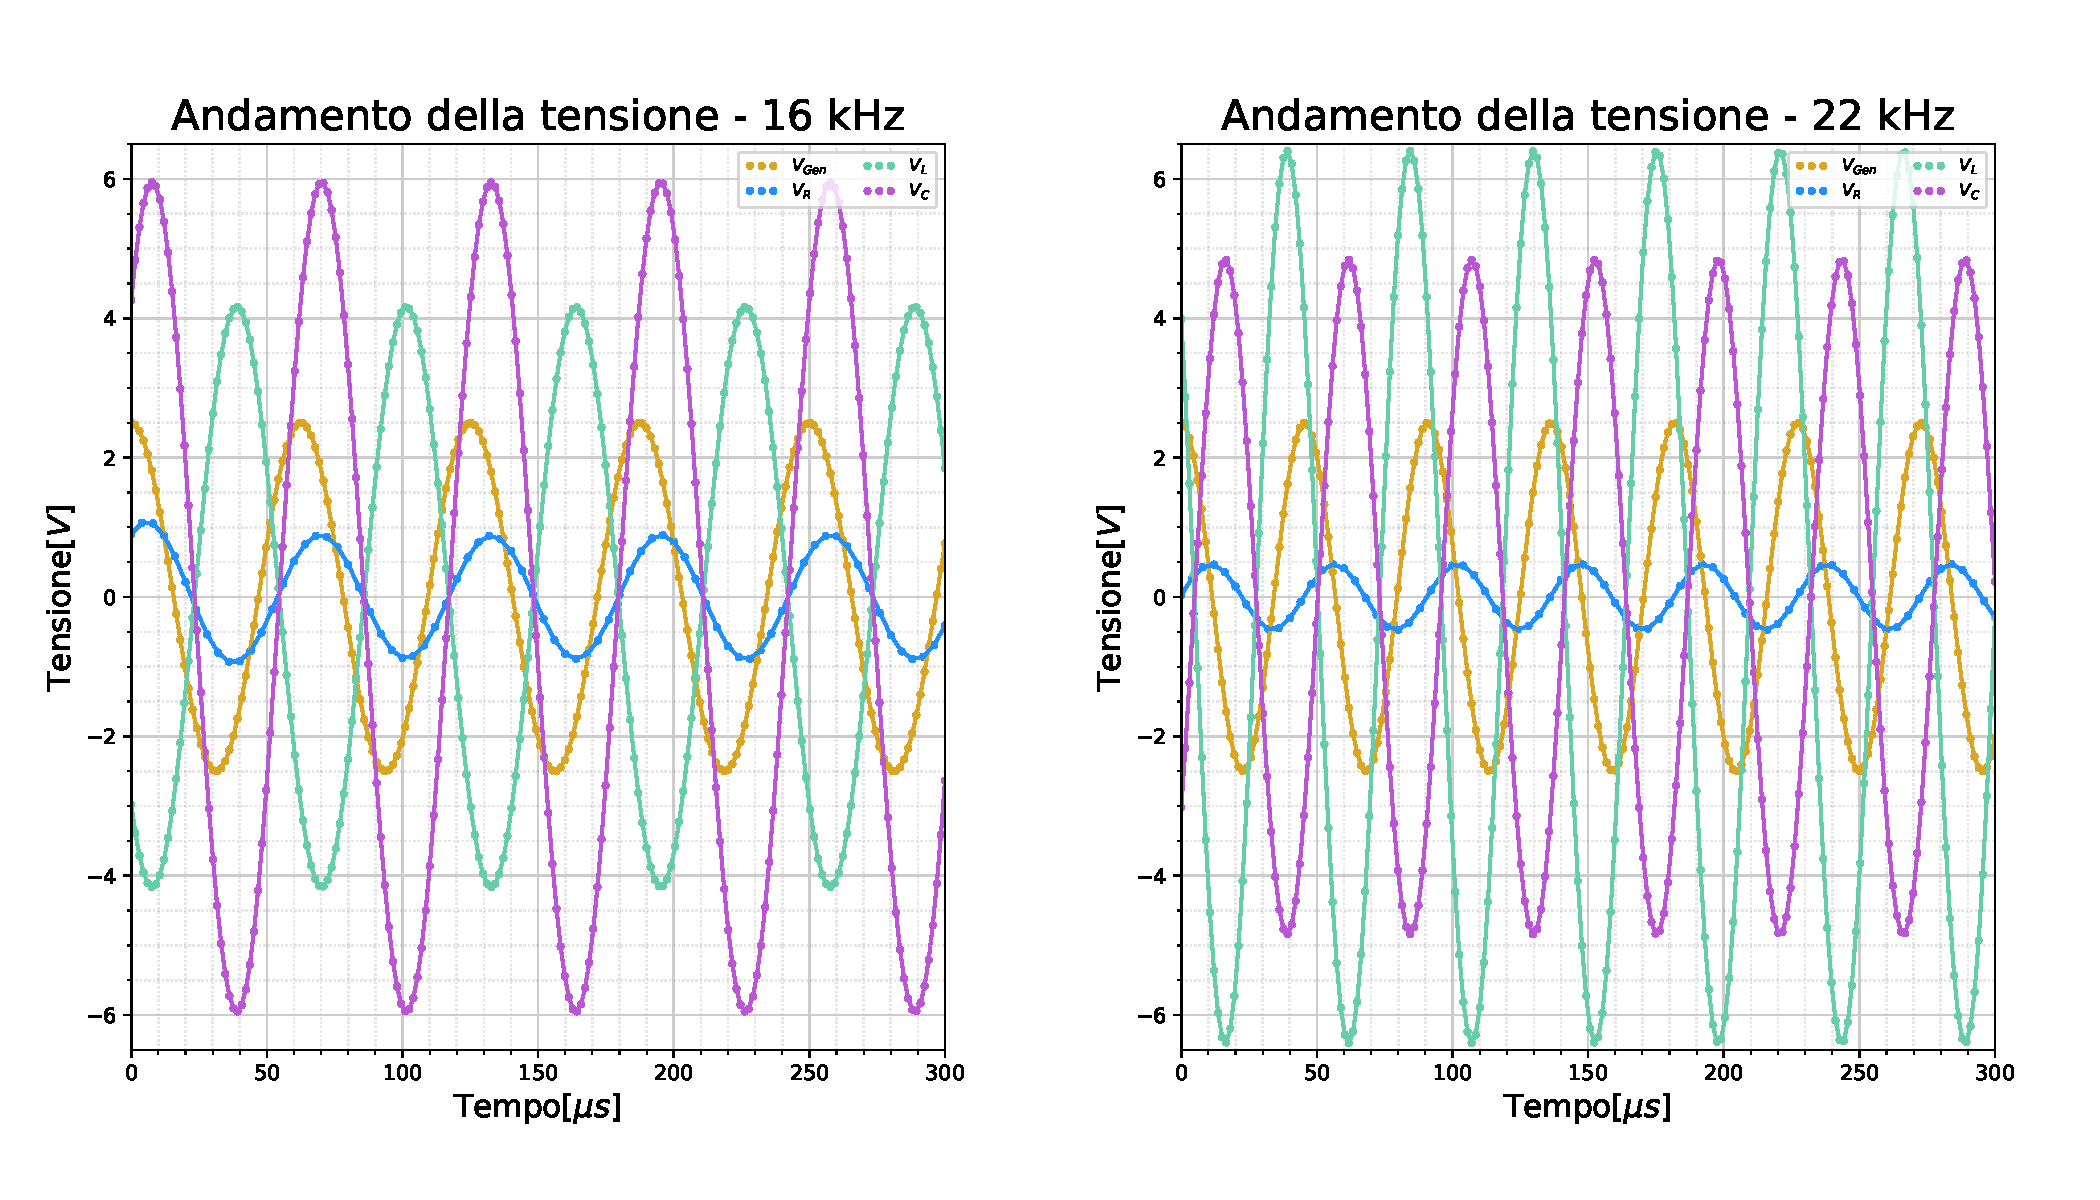
\includegraphics[width=1\textwidth]{../figs/tensione-tempo.pdf}
    \caption{\emph{I grafici mostrano gli andamenti della tensione ai capi dei vari componenti quando il generatore
    oscilla ad una frequenza di $f=16kHz$ e di $f=22kHz$; questi sono valori prossimi a quelli che definiscono la banda del filtro.}}
    \label{fig:tensione-tempo}
\end{figure}

%#TODO scrivere che la risposta infrequenza viene fatta grazie al function genrator di elvis

Una volta realizzato il circuito, ne è stato valutato il comportamento qualitativo. A tal proposito si è valutato visivamente
l'andamento temporale delle differenze di potenziale sui vari elementi circuitali mediante l'utilizzo dell'oscilloscopio digitale disponibile in
laboratorio.
In secondo luogo, per una valutazione a posteriori, sono stati raccolti tali dati tramite la DAQ configurata.
Ciò è stato fatto mantenendo la frequenza del generatore costante. In figura \ref{fig:tensione-tempo} sono
mostrati tali andamenti per due valori significativi di $f$ in quanto vicini ai valori di taglio della frequenza, caratteristici
di questo circuito.
%#TODO commento su come ampiezze della tensione hanno senso e anche la fase dopo la risonanza
l’andamento della tensione sulla resistenza è risultato essere in fase con quello indotto sul generatore, come ci si
aspettava dal punto di vista teorico.

%%%%%%%%%%%%%%%%%%%%%%%%%%%%%%%%%%%%%%%%%%%%%%%%%%%%%%%%%%%%%%%%%%%%%%%%%%%%%%%%%%%%%%%%%%%%%%%%%
%%%%%%%%%%%%%%%%%%%%%%%%%%%%%%%%%%%%%%%%%%%%%%%%%%%%%%%%%%%%%%%%%%%%%%%%%%%%%%%%%%%%%%%%%%%%%%%%%
%%%%%%%%%%%%%%%%%%%%%%%%%%%%%%%%%%%%%%%%%%%%%%%%%%%%%%%%%%%%%%%%%%%%%%%%%%%%%%%%%%%%%%%%%%%%%%%%%
\subsection{Analisi delle ampiezze}

Quella che segue è l'analisi della risposta in frequenza del circuito.
I dati relativi alle ampiezza della tensione ai capi dei vari elementi, sono visibili in Figura \ref{fig:ampiezzeRLC}
dove sono stati riportati anche i fit secondo i modelli ipotizzati.

\begin{figure}[h]
    \centering
    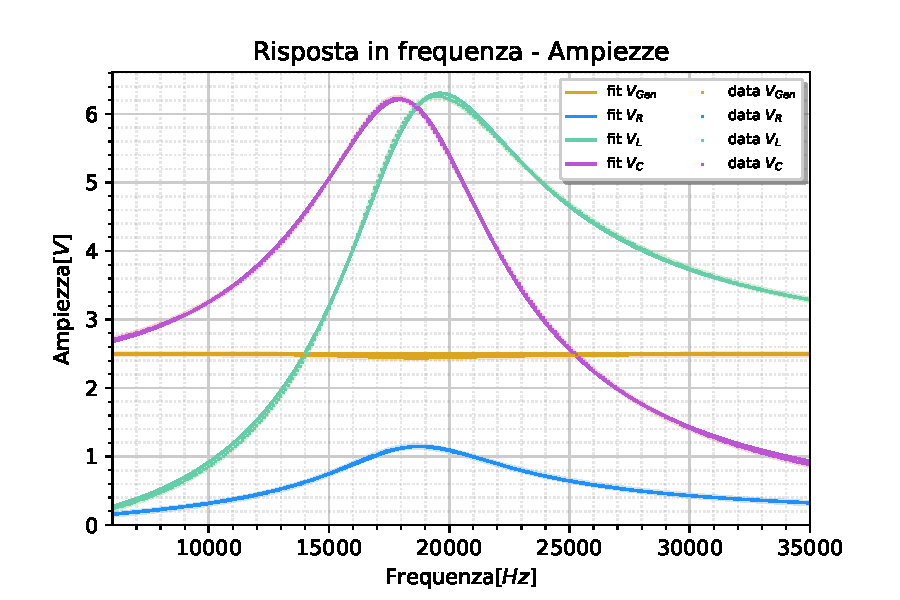
\includegraphics[width=1\textwidth]{../figs/Risposta-in-frequenza-ampiezze.pdf}
    \caption{\emph{Andamento dell’ampiezza della tensione sulle componenti del circuito al variare
    della frequenza del generatore con sovrapposte relative curve best-fit.}}
    \label{fig:ampiezzeRLC}
\end{figure}
Non conoscendo in maniera precisa il funzionamento del subVI 'Extract singleton information', che ha fornito le misurazioni
di ampiezze e fasi, è stato scelto di stimare le incertezze su tali dati tramite il rumore di fondo. E stata quindi
calcolata la deviazione standard delle misure associate all’ampiezza della tensione agli estremi, che sono posti
come costanti, ottenendo $\sigma = 3.9 10^{-3} Hz$

Gli andamenti attesi per le varie ampiezze della tensione sono i seguenti(vedi Appendice):

\begin{equation}\label{eq:amp-V_R}
    V_R = \frac{R_rV_0}{\sqrt{ R^2 +{ \left(\omega L - \frac{1}{\omega C}\right)}^2}}
\end{equation}
\begin{equation}
    V_L = \frac{\omega L V_0}{\sqrt{R^2+{ \left(\omega L - \frac{1}{\omega C}\right)}^2}}
\end{equation}
\begin{equation}
    V_C = \frac{\frac{V_0}{\omega C}}{\sqrt{R^2+{ \left(\omega L - \frac{1}{\omega C}\right)}^2}}
\end{equation}


\begin{figure}[h]
    \centering
    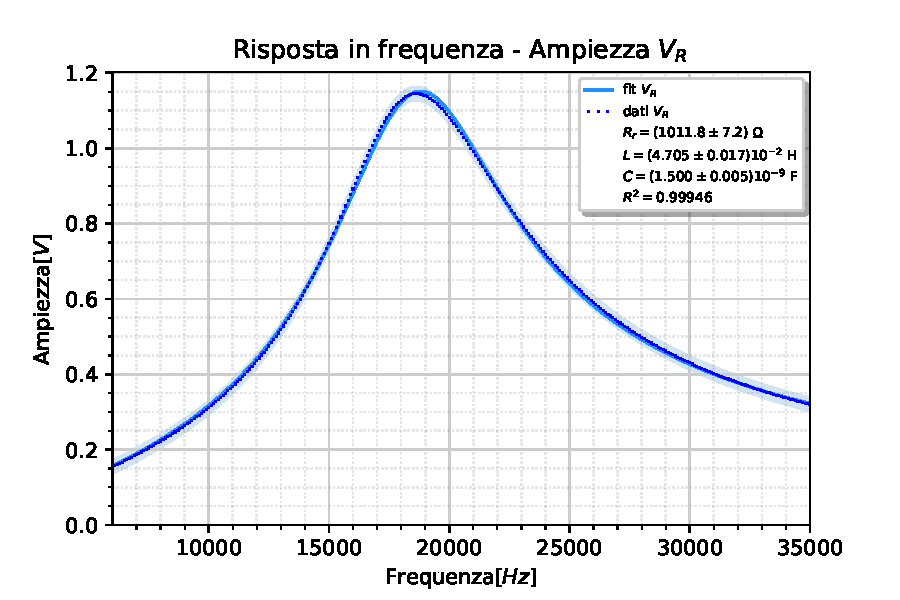
\includegraphics[width=.9\textwidth]{../figs/Risposta-in-frequenza-ampiezza-resistenza.pdf}
    \caption{\emph{Il grafico mostra in dettaglio l'ampiezza della tensione sul resistore, con sovrapposto relativo fit
        (equazione \ref{eq:amp-V_R}).}}\label{fig:ampiezzeR}
\end{figure}

Si è distinto tra il valore della resistenza del resistore stesso,$R_r$, e quello della resistenza totale opposta nel
circuito, $R$.
Da una prima analisi dei dati è stato verificato l'andamento caratteristico del filtro, con le ampiezze massimizzate
in corrispondenza di un valore specifico di frequenza.

%#TODO scrivere diversametne questa cosa
%Osservando qualitativamente il grafico, da esso si nota una leggera diminuzione dell’ampiezza della tensione indotta
%nel circuito in valori prossimi a quello stimato come di risonanza. Cio` si spiega con la presenza della resistenza
%interna del generatore, che provoca una caduta di potenziale tanto maggiore quanto lo `e la corrente, che si sa essere
%massima proprio in condizioni di risonanza.
Dai fit sono emersi valori del $\tilde{\chi}^2$ piuttosto elevati. Questo è dovuto ad una sottostima della valutazione
dell'incertezza sui valori di ampiezza di $V$. Si è, pertanto, scelto di utilizzare come indice della goodness-of-fit
il cosiddetto coefficiente di determinazione $R^2$.
Il fit più significativo è risultato essere quello dell'ampiezza di $V_R$, mostrato in Figura \ref{fig:ampiezzeR}, con
un valore di $R^2 = 0.99946$. Da tale fit i valori dei componenti risultano essere $R_r = (1011.8 \pm 7.2) \ \Omega$,
$L = (4.705 \pm 0.017)10^{-2}$ e $C = (1.500 \pm 0.005)10^{-9}$ F. Si è scelto di utilizzare le "incertezze
standard" calcolate come
\[
    \delta p_k = \sqrt{\tilde{\chi}^2 C_{kk}}
\]
dove $C_kk$ è l'elemento corrispondente a $p_k$ nella diagonale della matrice di covarianza.

Si e valutata la frequenza di risonanza con i parametri ottenuti dal fit associato alla resistenza usando l'equazione
\ref{eq:res-pulsation} ottenendo $f_0 = (18.95 \pm 0.05) kHz$, con le incertezze propagate in quadratura.

In secondo luogo, studiando il massimo dell'ampiezza di $V_R$, si è stimato un range di valori centrato in
una certa frequenza $f$ che corrisponde teoricamente a quella di risonanza, per quanto detto in precedenza.


Preso l’estremo inferiore della barra di errore relativa al punto di massimo estratto dal fit, si sono poi cercati i
punti in cui l’estremo superiore della barra di errore corrispondesse a tale valore massimo. In questo modo, però, si
è sovrastimata l’incertezza relativa alla frequenza di risonanza, calcolandola come il valore medio di questi due estremi.
Da tale procedura si è ottenuto un valore $f_0 = (18.80 \pm 0.28)kHz$.
La significatività di tale risultato è ridotta, avendo utilizzato una sovrastima dell'incertezza.

%#TODO SCRIVERLO NOSTRO
Un'anamolia emersa dall'analisi dei dati raccolti riguarda il valore della resistenza totale del circuito, che, dai fit
dei dati raccolti risulta sempre essere largamente superiore al valore teorico. In Appendice si analizza meglio questa
evenienza.

%%%%%%%%%%%%%%%%%%%%%%%%%%%%%%%%%%%%%%%%%%%%%%%%%%%%%%%%%%%%%%%%%%%%%%%%%%%%%%%%%%%%%%%%%%%%%%%%%
%%%%%%%%%%%%%%%%%%%%%%%%%%%%%%%%%%%%%%%%%%%%%%%%%%%%%%%%%%%%%%%%%%%%%%%%%%%%%%%%%%%%%%%%%%%%%%%%%
%%%%%%%%%%%%%%%%%%%%%%%%%%%%%%%%%%%%%%%%%%%%%%%%%%%%%%%%%%%%%%%%%%%%%%%%%%%%%%%%%%%%%%%%%%%%%%%%%
\subsection{Analisi delle fasi}

Le funzioni che descrivono gli andamenti attesi delle fasi sono le seguenti:
 \[
     \phi_R = \arctan{\frac{1 - \omega^2 L C}{R \omega C}}
 \]
\[
    \phi_L = \arctan{\frac{1 - \omega^2 L C}{R \omega C}} + \frac{\pi}{2}
\]
 \[
     \phi_C = \arctan{\frac{1 - \omega^2 L C}{R \omega C}} - \frac{\pi}{2}
 \]

\begin{figure}[h]
    \centering
    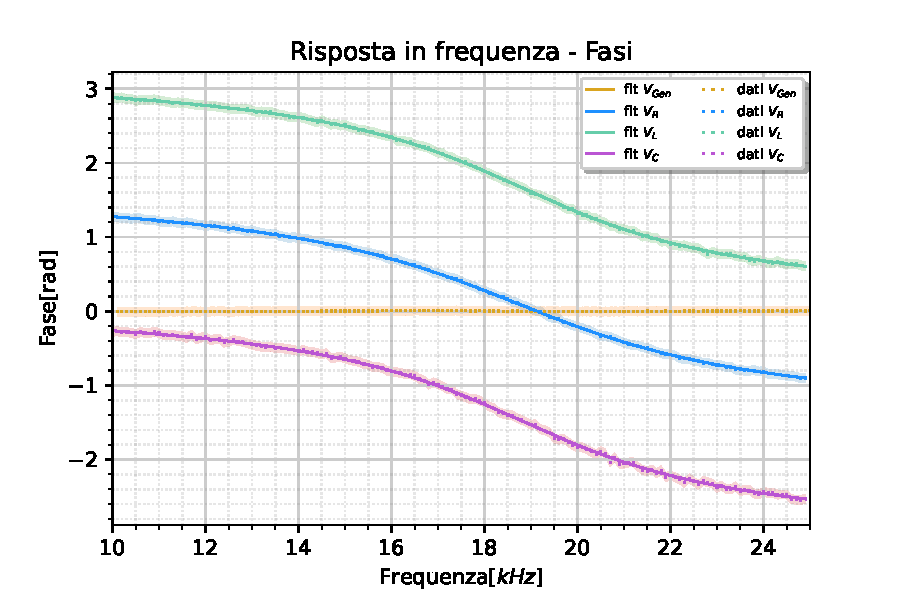
\includegraphics[width=.9\textwidth]{../figs/Risposta-in-frequenza-fasi.pdf}
    \caption{\emph{Andamento dello sfasamento della tensione sulle componenti al variare della frequenza del generatore.}}
    \label{fig:fasi}
\end{figure}

I dati sullo sfasamento della tensione sonostati raccolti in concomitanza con quelli sulle ampiezze. È stato scelto di
sottrarre ai dati sulle fasi di $R, L , C$ i corrispondenti valori di $\phi_{\text{gen}}$ in quanto quello che
si dovrebbe misurare è lo sfasamento rispetto al generatore.
In figura \ref{fig:fasi} sono visibili tali dati assieme alle curve best-fit, ottenute considerando solamente i valori
fra $10  \ \text{e} \ 25 kHz$ con un valore caratteristico di $R^2 = 0.986$. Il rumore di fondo è stato valutato in
maniera analoga a quanto fatto per le ampiezze, estraendo la deviazione standard degli sfasamenti a $f$ costante,con
$\sigma_{\phi} = 0.002$ rad.
Considerando la curva associata alla resistenza, si è pensato di estrarre il punto della funzione ottenuta dal
fit di valore nullo e stimare un range, definito dalla barra di errore. Il valore corrispondente a quando questa curva si trova ad avere fase nulla con il generatore
è quindi $f_0 = (19.10 \pm 0.10)kHz$, prossimo al valore atteso. Ripetendo il procedimento con la curva dell’induttanza,
ma stavolta cercando uno sfasamento di $\frac{\pi}{2}$, si è avuto nuovamente un esito vicino ai precedenti, ovvero
$f_0 = (19.35 \pm 0.15)kHz$.

%#TODO valuta se scrivere del ritardo ecc...






















 \section{Conclusione}
  

In conclusione il comportamento del filtro è risultato essere in accordo con la teoria.
Per quanto riguarda il fenomeno della risonanza, dall'analisi delle ampiezze per $f_0$ sono stati
ottenuti i valori $f_0 = (18.95 \pm 0.05) kHz$ e $f_0 = (18.80 \pm 0.28)kHz$, mentre
da quella delle fasi $f_0 = (19.10 \pm 0.10)kHz$ e $f_0 = (19.35 \pm 0.15)kHz$ .
Si è ipotizzato che le discrepanze dal valore atteso  $f_0 = (19.13 \pm 0.14) kHz$, dove presenti, siano dovute ai diversi fattori ambientali, primo fra tutti la temperatura
variabile delle componenti della scheda di acquisizione NI ELVIS II, fenomeno dovuto all’effetto Joule.

È stata inoltre evidenziata un'errata stima iniziale della resistenza totale del circuito, in quanto i valori di tale
grandezza sono risultati sistematicamente superiori in tutti i fit realizzati.
Per avere un'idea di quanto tale valore risulti superiore a quello atteso, $R_{\text{tot}} = (1172.5 \pm 1.6) \ \Omega$, si riporta
$R =( 2.15 \pm 0.15 )10^3 \ \Omega$, dato ottenuto nel caso del fit, piuttosto significativo, dell'ampiezza di $V_R$.

 \section{Appendice}
   Come si può notare in Figura 6. le ampiezze nei primi periodi presentano dei picchi più elevati per poi stabilizzarsi a un valore massimo costante, questo comportamento però risulta essere anomalo dal momento che il circuito analizzato in questa esperienza di laboratorio non ha le caratteristiche tipiche di un transiente.
Si è cercato, perciò, di risolvere l’anomalia ripetendo le misure con componenti equivalenti, senza però ottenere nessun risultato positivo nella risoluzione del problema. (L’ho scritto perchè sembra una cosa logica anche se non l’abbiamo fatta).
Dopo vari tentativi, si è ipotizzato che questa anomalia sia dovuta al modo in cui sono raccolti i primi dati dal programma di acquisizione Labview, in particolar modo si è pensato che il problema potesse essere dovuto al trigger del software.

Al fine di studiare il comportamento del circuito analizzato in questa esperienza di laboratorio, si è utilizzato il concetto di impedenza, che generalizza il concetto più specifico di resistenza nel caso di correnti sinusoidali.
L’impedenza totale è data dalla somma delle impedenze di ciascun componente, sfruttando il fatto che questi siano posti in serie. Perciò avremo...


dove j indica l’unità immaginaria, mentre il termine tra parentesi indica la reattanza, costituita in parte dal contributo induttivo e in parte da quello capacitivo.
Per trovare la corrente nel circuito invece è stata applicata la legge di Ohm simbolica, sfruttando il formalismo dei fasori e, moltiplicando poi il valore ottenuto per l’impedenza ai campi di ciascun componente, si può trovare l’andamento della tensione su di essi.



 \end{document}

